\documentclass[a4paper]{article}

\usepackage[english]{babel} \usepackage[utf8x]{inputenc}
\usepackage{amsmath}
\usepackage{graphicx}
\usepackage[colorinlistoftodos]{todonotes} \usepackage[margin = 1.2in]{geometry}

\title{A Bug's Life}
\author{Oliver Eriksson Edholm (XXXXXX-YYYY) \\
Aleksander Lundqvist (XXXXXX-YYYY) \\
Henrik Sommerland (890618-4950) \\
Edvin Wahlberg (XXXXXX-YYYY) \\
Oscar Wallster(910615-1096)}

\begin{document}
\maketitle

\section{Introduction}
% This could be rewritten in a far more persuasive manner
We have decided that we are going to simpulate an \emph{ant ant}. We want to do
this in order to learn more about both \emph{swarm intelligence} and the actor
model.\\
We choose ants in inspiration of their ability to cooperate in a very large
scale and solve complex problems while still every ant is only following very
simple rules.
\\
Our goal is not to simulate the behaviour of real world ants or to mimick the
datails of any biological systems.
We are more interested in the theorethical concepts of how complex behaviors can
arise from the interaction of a large group of agent each possesing only limited
cognitive abilites.\\

One of the later goals is also to have two or more ant hives interact with
eachother in a world where food is scarce, and battles are inevidieble.

\subsection{Chalenges}

\subsubsection{Concurrency}
Making heavy use of the actor model using thousands of actors will create a lot
of complexity and there are many posibilities for problems to occur. The most
obvious danger is the possibilty of deadlocks to occur. With many actors
comunicating together one is almost certain that one will get some form of
circular dependencies. So great care needs to be taken to ensure that no
deadlocks will occur.

There is also a risk of severe performance degradation in regions with many
interacting actors. Although this is something wich is intrinsic to the actor
model and it may be hard for us to control it.

\subsubsection{Rules For Interaction}
The other chalange will be to setup rules for how the ants interact with the
world and jhow the world gets updated. The parameters for these rules will need
to be finetuned and it may be hard to find rules which result in complex
behaviours. It is also very hard to analytically determine these parameters so
the only feasible alternative is to trough experimentation find rules which
yields satisfactory behavious.

\subsubsection{Social Challanges}
In order to get this project moving forward in a pace that is required, we need
to have every member of the group working regularly certain hours of the weeks.
In order to achieve this every member needs to have the same mental image over
the finished project, therefore we need to be active with communication in the
roup so that noone is left behind and wonders what he could/should be doing.

\section{Concurrency Models and Programming Languages}

\subsection{Concurrency Goals}
As previously stated we want to create a system wich relies heavily on the actor
model. Our project idea is well suited for this since the ants are by nature
individual agents who and make decisions without any direct knowlegde of the
global state.

We want to make our simulation free of so called \emph{stop the world}
sencarios. These are when we for some reason have to block al of the actors in
the simulation in order to perform some kind of action.

\subsection{Language Requirement}
Our main requirement for the programming language we choose is that it have to meet our concurency goals.
We have discarded c/c++ because it's to lowlevel and we would have to implement the actor model ourself. 
Also java because it's not the proper concurrency model. We are considering python for frontend(graphics),
but it's not suited for our backend needs.

\subsection{Rust}

\subsection{Nim}

\subsection{Erlang}

\subsection{Encore}

\section{System Architecture}

\begin{figure}[h!]
\centerline{
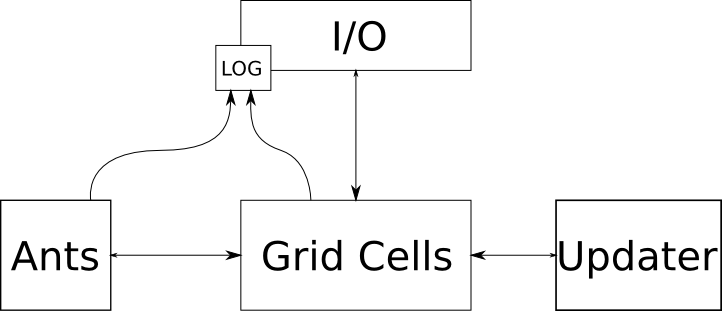
\includegraphics[scale=0.6]{images/architecture.png} 
}
\caption{A draft of a system architecture} 
\label{fig:arch}
\end{figure}
Above you can see a rough draft of the architecture of the system. EAch box
represents an agent, note that this i just a conceptual map of the
communication between the different agents. The arrows between the a means that
they comunicate via message passing.
The large arrow indicates that a message will be sent between those actors in that
direction. The smaller awrrows on the liness indicates that the sending actor
will block untill a reply message is recieved.

\subsection{Ants}
In figure~\ref{fig:arch} the box labled \textbf{Ants} corresponds to the ant
object.
The ant will be an independet actor holding very little infromation about its
own state but containing the faculties to make descisions based on recieved
input. The ant actor will send a message to the cell querrying about the state
of its neighbouring cells. The ant will then wait for the reply message from its
cell and then take some action based on the reply from the cell. the actor then
sends a message to its cell requesting to do whatever it is that the ant wanted
to do and then awaits a reply weather or not the move was successfull.

\subsection{Grid Cell}
In figure~\ref{fig:arch} the box labled \textbf{Grid Cells} corresponds to one
cell on the ``map''. Each of these cells contains all the information about the state of
that cell. It also contains references to its neighbouring cells in order to
retrive the information about its neighbourhood. The cell will wait for querrys
from ants to recive the state of the neighbourhood and the cell will also
process requests from ants to perform actions such as moving or picking up food.

\subsection{Updater}
In figure~\ref{fig:arch} the box labled \textbf{Updater} is something that will
handle the background work for the cells. Such as the dissipation of the feremones.We
are uncertain weather or not to use this approach with a seperate actor sweeping
trough all of the cells and updating them. We could let each of the cells handle
their own ``passive'' updates but that might result in performance degredation
since the cells would either always be doing work or we might need to introduce
some form of delay.

\subsection{I/O}
In figure~\ref{fig:arch} the box labled \textbf{I/O} is the actor that be
responsible for the handling of the input and output. this actor will sweep thrugh the cells and
querry them for their state and then process output the information in some
suitable fashion. We may add support for some form of interactivity at a later
state.

\subsection{LOG}
In figure~\ref{fig:arch} the box labled \textbf{LOG} will be a simple actor wich
is just waiting for logging mesages from the ants and the grid cells. This will be
used as a form of rudimentary output and for debugging purposes.


\section{Development Tools}
Communication and planning: To plan meetings and set up to-do tasks for the
project, we have chosen to use Trello. Trello is a very user friendly and will
give us a great overview of the progress of the project. It will also be a good
tool to keep track of who is doing what. For communication we’re going to use
Slack to ensure that we have all communication of the project in one place. If
we should have chosen to use Facebook it’s very easy to get distracted and talk
about other things that isn’t related to the project. If we really need to discuss
something urgent we’re going to use Skype. Working in a group of six fully active members
it is very important that everyone in the group keeps himself up-to-date with the progress. 
We were therefore very carefull when choosing the communication medias so that everyone would
feel that they would check the media every day. Again, the problem with facebook is that 
although everyone would check it daily, there would be a lot of other things going on.
The communication environment needs to be strictly for work related things to keep everyone
focused on what's important. 


\section{Conclusion}
Digital ant colonization is perfect project for developing deeper understanding
of the actor model of concurency, since each ant is an independent actor and
only interact with its immidiate surroundings. This project can be divided into
diffrent milestones which can be developed further as time lasts. We all have
alot and diffrent ideas how we want the final product to work, but we all agree
on the basics so as time elapse we will hopefully be able to add alot more
complexity depending how much work will be needed for each milestone. Ergo we
start with a stable core and build outwards in diffrent directions.
\end{document}

